% Chapter 2
\chapter{RELATED WORK} % Chapter Title in ALL CAPSacs
This chapter gives a survey of the possible approaches to Spam Filtering. We proposed to use a semantic similarity approach, which involved the construction of a latent semantic feature space and a corpus based thesaurus. The output of each email must contain a classification- either ‘Spam’ or ‘Ham’. This survey helped us analyse the various existing approaches to Spam Filtering and decide on the one which would best cater to our needs. 

\section{NAIVE BASED APPROACH}

This approach involves the application of the famous Bayes’ Probability Theorem in the domain of Spam Filtering \cite{1}.  Bayes’ Theorem can be stated as follows:

$P(H|E)=(P(H)*P(E|H))/P(E)$

In the above equation,


\textbf{$ P(H|E)$} : Posterior probability of ‘H’ , given evidence ‘E’


\textbf{$ P(H)$} : Prior probability


\textbf{$ P(E|H)$} : Likelihood of evidence ‘E’ if hypothesis ‘H’ is true


\textbf{$ P(E)$} : Priori probability that the evidence itself is true

The above formula is used to calculate the probability that an item belongs to a certain class. Suppose that we knew exactly, that the word DISCOUNT could never occur in a legitimate message. Then when we saw a message containing this word, we could tell for sure that it was spam. This simple idea can be generalized using some probability theory. We consider two categories classes: Spam(S) and Ham (H). For a given message x,

If $(S|x)>P(H|x)$ , (that is, if the a-posteriori probability that x is Spam is greater than the a-posteriori probability that x is non-spam), classify x as Spam, otherwise classify it as Ham.

This can be transformed to the form: If  $((P(x|S)/P(x|H))>(P(H)/P(S)))$ , classify x as Spam, otherwise classify x as Ham.
Consider a message ‘m’ containing a feature vector ‘x’. Let us try the simplest case of a feature vector with a single binary attribute that denotes the presence of a certain word ‘w’ in the message. The message’s feature vector x is set to 1 if the word is present in the message, 0 otherwise.

The decision rules are then used to classify a given message as Spam or Ham. This approach however assumes predictors are independent \citep{2}. In real life, it is almost impossible that we get a set of predictors which are completely independent.

\section{K-NEAREST NEIGHBOURS}
The k-nearest neighbour (K-NN) classifier is considered an example-based classifier, which means that the training documents are used for comparison rather than an explicit category representation, as in the case of the Naïve Bayes’ approach. This approach is generally considered as amongst the simpler machine learning algorithms.
When a new object needs to be categorized, the k most similar objects (neighbours) are found and if a large enough proportion of them have been assigned to a certain category, the new object is also assigned to this category, otherwise not.\citep{3} If k = 1, then the object is simply assigned to the class of that single nearest neighbour. 

\begin{figure}[h]
\centering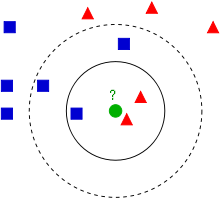
\includegraphics[width=0.75\linewidth]{knn.png}\caption{An example showcasing the K-Nearest Neighbours and their polling}
\end{figure}

The test sample (green circle) should be classified either to the first class of blue squares or to the second class of red triangles. If k = 3 (solid line circle) it is assigned to the second class because there are 2 triangles and only 1 square inside the inner circle. If k = 5 (dashed line circle) it is assigned to the first class (3 squares vs. 2 triangles inside the outer circle).
In the context of Spam Filtering, given a message x, we need to first determine its k nearest neighbours among the messages in the training set. If there are more spam's among these neighbours, the message is classified as Spam. Otherwise, it is Ham.
One of the drawbacks of the presented algorithm is that there seems to be no parameter that we could tune to reduce the number of false positives. This problem is easily solved by changing the classification rule to the following l/k-rule:

If l or more messages among the k nearest neighbours of x are spam, classify x as spam, otherwise classify it as legitimate mail.

\section{ENSEMBLE FILTERING WITH ACTIVE LEARNING}
Ensemble learning methods typically use a large number of classifiers. When a new sample is to be classified, a combination of results produced by each single classifier governs the overall classification of the sample.
In active learning, a small number of labelled training samples are used to build an initial classifier. The basic idea of selecting samples takes into account the roles of different samples in classification, namely, the greater the amount of information contained in samples, the more important they are in the determination of the classification surface. That is to say, for a large number of unlabelled samples, only a few of them need to be labelled and used to train the model with strong classification performance.
Pool-based active learning methods have achieved good results in spam filtering with only a few e-mails tagging. A Pool-based active learning method assumes that the learner can access to n unlabelled samples and at most m (m << n) of them can be requested when it needs user tagging \citep{4}. Researchers have made a wide range of approaches to obtain m samples, among which there are two typical methods: uncertainty sampling based method and query by committee based method \citep{5}. The former one is to select samples, in which the filter is unable to clearly distinguish to join the training set and then use these samples to train classifier. The latter one is to build two or more classifiers based on history labelled samples as “committee”, then make use of the committee to vote on incoming samples and the samples with most inconsistent votes are selected as candidates for training.

\section{BOOSTING TREE APPROACH}
Boosting is an ensemble technique that attempts to create a strong classifier from a number of weak classifiers. This is done by building a model from the training data, then creating a second model that attempts to correct the errors from the first model. Models are added until the training set is predicted perfectly or a maximum number of models are added.\citep{6}

\section{OBSERVATIONS FROM THE SURVEY}

We propose to incorporate a semantic- similarity based approach to spam filtering. Therefore, it no single approach mentioned above will fit the given bill.  Other traditional and common spam filtering methods, such as Backpropagation Neural Networks (BPNN) and Vector Space Modelling (VSM) also have their own drawbacks. For example, neural networks have the problems of slow training speed and easy to trap into local minima. Vector space model has three challenges: high dimensionality, sparse representation and semantic concern. For our approach, we have chosen to implement a Latent Sematic Feature Space (LSFS) and a Corpus Based Thesaurus (CBT). We use the standard implementations of Multi-Layer Perceptrons (MLPs) and Support Vector Machines (SVMs) for our classification purposes.
%% The Appendices part is started with the command \appendix;
%% appendix sections are then done as normal sections
%% \appendix

%% \section{}
%% \label{}


